%
% fig-ants.tex
%
% (c) 2025 Prof Dr Andreas Müller
%
\begin{figure}
\centering
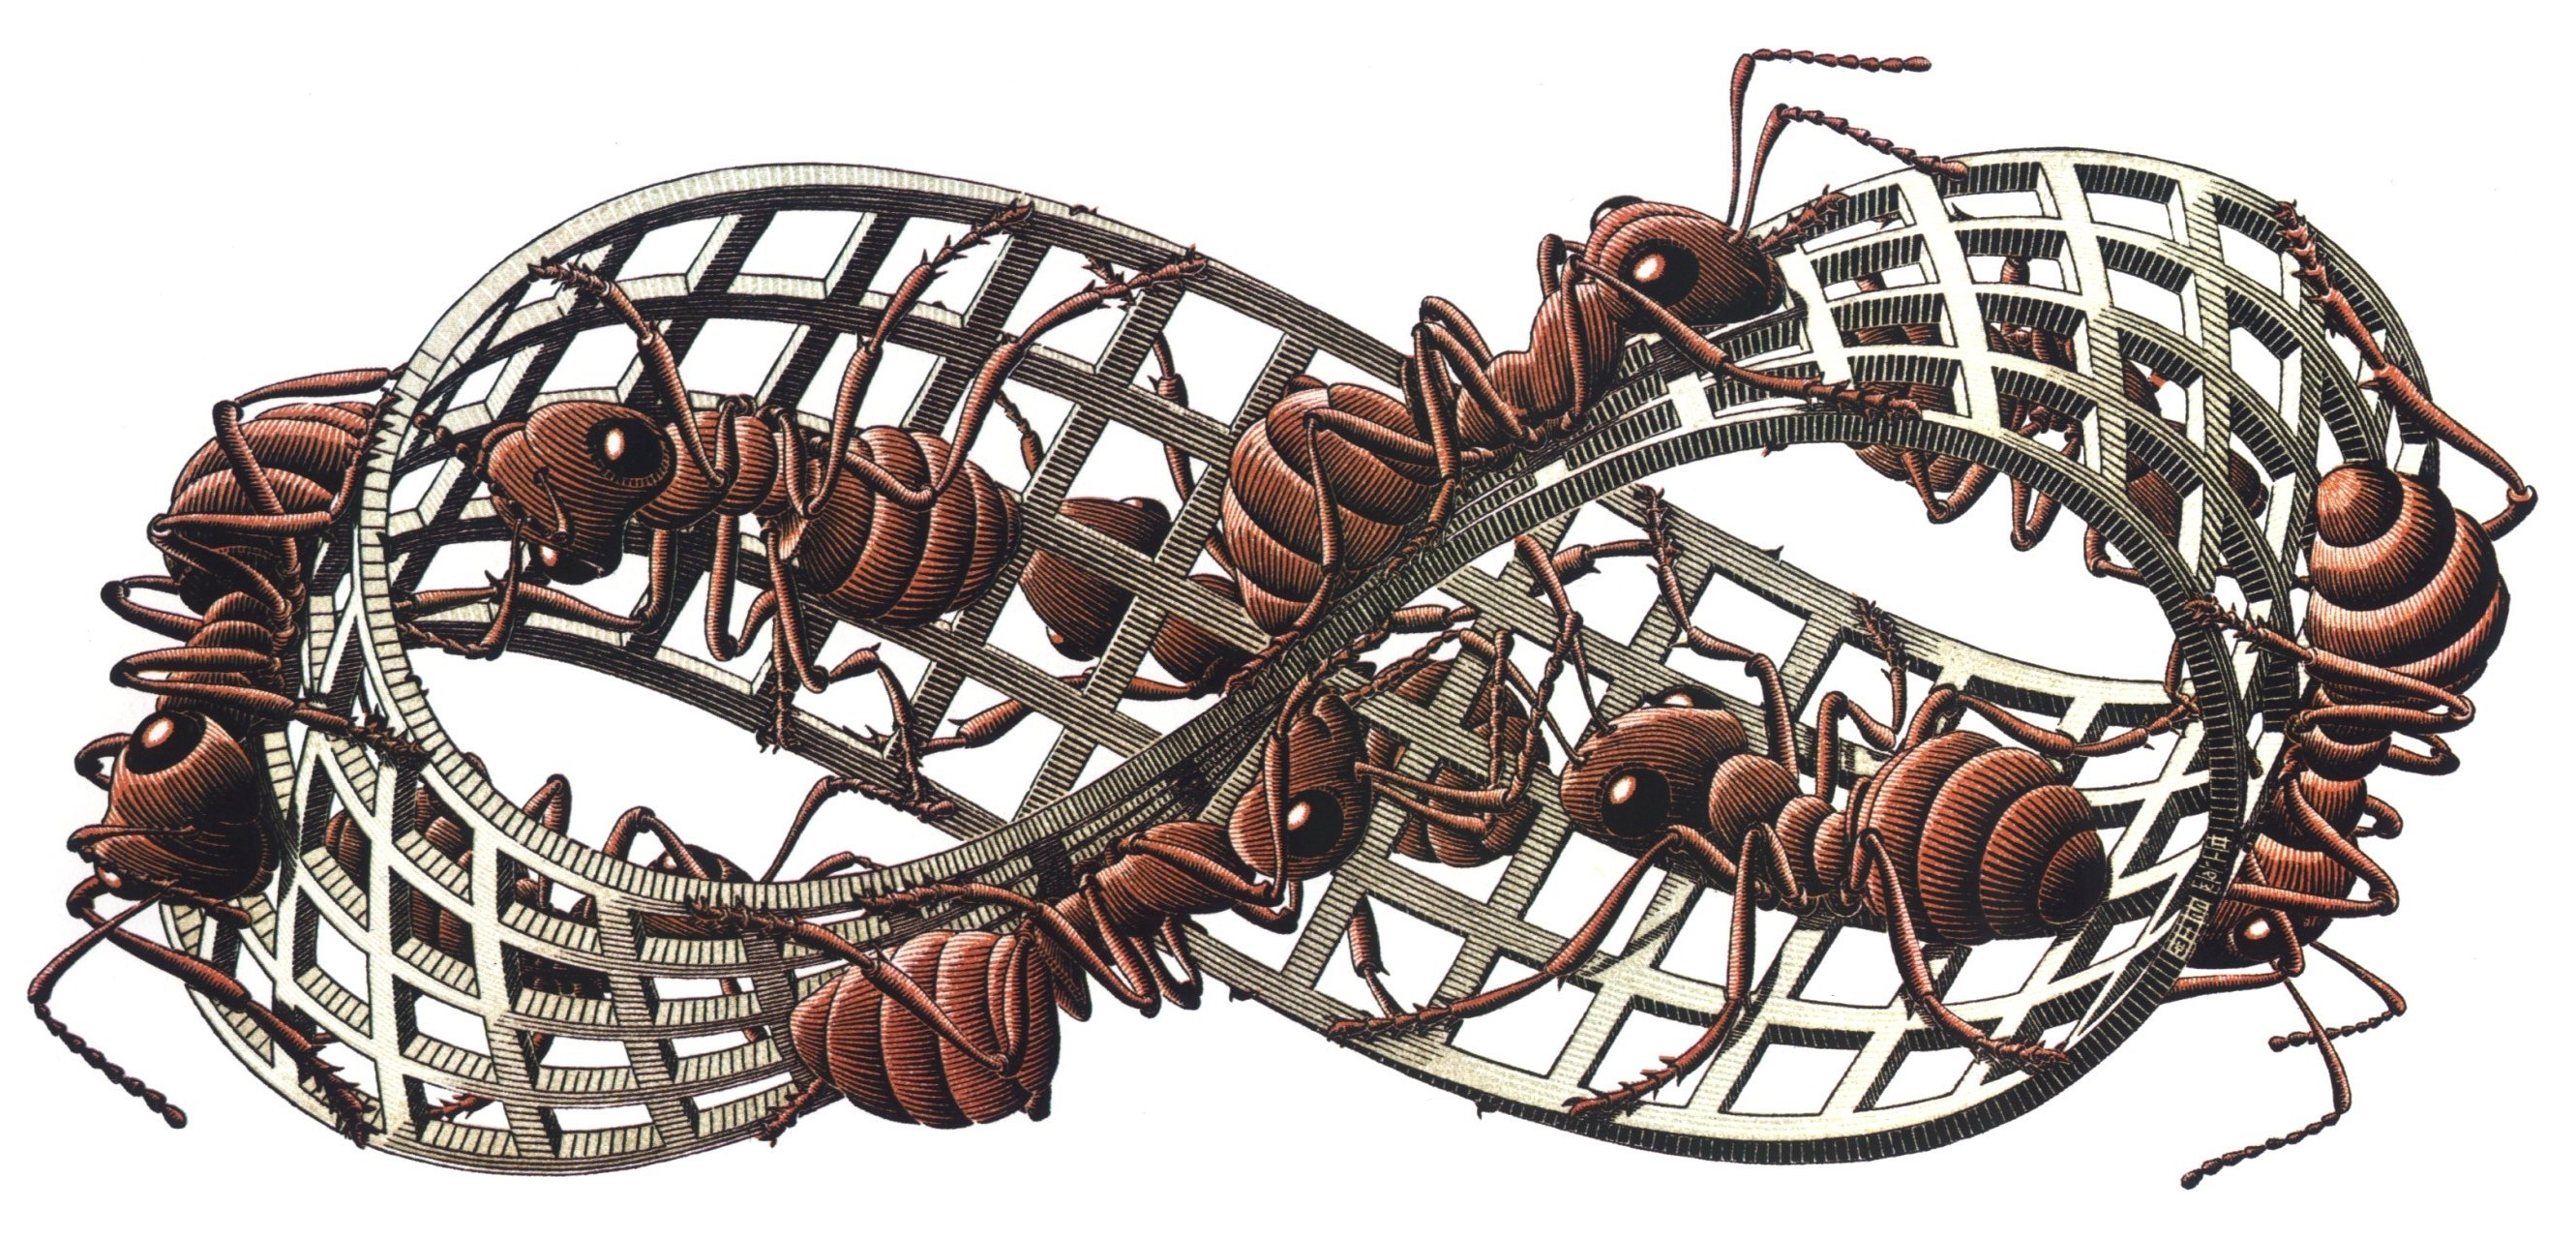
\includegraphics[width=\textwidth]{chapters/040-green/images/ants.jpg}
\caption{Krabbelt eine Ameise auf einer Seite eines Möbius-Bandes,
findet sie sich nach einem Umlauf auf der anderen Seite wieder, da
das Möbius-Band eine nicht orientierbare Mannigfaltigkeit ist.
(Stich von M.~C.~Escher)
\label{buch:green:fig:ants}}
\end{figure}
